
\documentclass[11pt]{article}
\usepackage{amsmath,amssymb,amsfonts} 
\usepackage{epsfig} \usepackage{latexsym,nicefrac,bbm}
\usepackage{xspace}
\usepackage{color,fancybox,graphicx,subfigure,fullpage}
\usepackage[top=1.25in, bottom=1.25in, left=1in, right=1in]{geometry}
\usepackage{tabularx} \usepackage{hyperref} 
\usepackage{pdfsync}
\usepackage[boxruled]{algorithm2e}
\usepackage{multicol}
\usepackage{enumitem}
\newcommand{\parag}[1]{ {\bf \noindent #1}}
\newcommand{\defeq}{\stackrel{\textup{def}}{=}}
\newcommand{\nfrac}{\nicefrac}
\newcommand{\opt}{\mathrm{opt}}
\newcommand{\tO}{\widetilde{O}}
\newcommand{\polylog}{\mathop{\mbox{polylog}}}
\newcommand{\supp}{\mathrm{supp}}
\newcommand{\rank}{\mathrm{rank}}
\newcommand{\ptot}{p_{\mathrm{tot}}}
\newcommand{\pmin}{p_{\mathrm{min}}}
\newcommand{\pmax}{p_{\mathrm{max}}}
\newcommand{\prob}[1]{\mathrm{Pr}\insquare{#1}}
\usepackage{algorithm}
\usepackage{algpseudocode}

\newcommand{\conv}{\mathrm{conv}}
\newcommand{\dist}{\mathrm{dist}}
\newcommand{\argmin}{\operatornamewithlimits{argmin}}
\newcommand{\sgn}{\mathrm{sgn}}
\newcommand{\fc}{\mathrm{fc}}


\newcommand{\cM}{\mathcal{M}}
\newcommand{\cB}{\mathcal{B}}
\newcommand{\cU}{\mathcal{U}}
\newcommand{\cY}{\mathcal{Y}}
\newcommand{\cF}{\mathcal{F}}
\newcommand{\capa}{\mathrm{Cap}}
\newcommand{\dcapa}{\underline{\mathrm{Cap}}}
\newcommand{\st}{\mathrm{s.t.}}
\newcommand{\un}{\mathrm{un}}

\newcommand{\Pb}{\mathbb{P}}
\newcommand{\sym}{\mathrm{sym}}
\newcommand{\pcount}{\mathbf{PCount}}
\newcommand{\mixdet}{\mathbf{MixDisc}}
\newcommand{\sbold}{\mathbf{S}}
\newcommand{\mb}{{M(\cB)}}

\newcommand{\mlb}{{M_{\mathrm{lin}}(\cB)}}
\newcommand{\redc}[1]{ \textcolor{red} {#1}}
\newcommand{\newt}{\mathrm{Newt}}
\newcommand{\wtf}{\widetilde{f}}
\newcommand{\wt}{\widetilde}
\newcommand{\diam}{\mathrm{diam}}
\newcommand{\lspan}{\mathrm{span}}
\newcommand{\interior}{\mathrm{int}}
\newcommand{\aff}{\mathrm{aff}}
\newcommand{\per}{\mathrm{per}}
\newcommand{\bl}{\mathrm{BL}}
\newcommand{\cE}{\mathbb{E}}


\newcommand{\eps}{\varepsilon}

\newenvironment{proof}{\noindent{\bf Proof:}\hspace*{1em}}{\qed\bigskip}
\clubpenalty=10000
\widowpenalty = 10000
\newcommand{\qed}{\hfill\ensuremath{\square}}


\def\showauthornotes{0} 
\def\showkeys{0} 
\def\showdraftbox{0}


\newcommand{\Snote}{\Authornote{S}}
\newcommand{\Scomment}{\Authorcomment{S}}

\newcommand\Z{\mathbb Z}
\newcommand\N{\mathbb N}
\newcommand\R{\mathbb R}
\newcommand\C{\mathbb C}

\newtheorem{theorem}{Theorem}[section]
\newtheorem{fact}{Fact}[section]
\newtheorem{conjecture}[theorem]{Conjecture}
\newtheorem{definition}{Definition}[section]
\newtheorem{lemma}[theorem]{Lemma}
\newtheorem{remark}[theorem]{Remark}
\newtheorem{proposition}[theorem]{Proposition}
\newtheorem{corollary}{Corollary}[section]
\newtheorem{claim}[theorem]{Claim}

\newtheorem{openprob}[theorem]{Open Problem}
\newtheorem{remk}[theorem]{Remark}
\newtheorem{example}[theorem]{Example}
\newtheorem{apdxlemma}{Lemma}
%\newtheorem{algorithm}[theorem]{Algorithm}
\newcommand{\question}[1]{{\sf [#1]\marginpar{?}} }

%% probability stuff

\newcommand\pr{\mathop{\mbox{\bf Pr}}}
\newcommand\av{\mathop{\mbox{\bf E}}}
\newcommand\var{\mathop{\mbox{\bf Var}}}

\newcommand{\ex}[1]{\av\left[{#1}\right]}
\newcommand{\Ex}[2]{\av_{{#1}}\left[{#2}\right]}

\def\abs#1{\left| #1 \right|}
\newcommand{\norm}[1]{\ensuremath{\left\lVert #1 \right\rVert}}



\newcommand{\tr}[1]{\mathop{\mbox{Tr}}\left({#1}\right)}
\newcommand{\diag}[1]{{\sf Diag}\left({#1}\right)}

\newcommand\set[1]{\left\{#1\right\}} %usage \set{1,2,3,,}
\newcommand{\poly}{\mathrm{poly}}
\newcommand{\floor}[1]{\left\lfloor\, {#1}\,\right\rfloor}
\newcommand{\ceil}[1]{\left\lceil\, {#1}\,\right\rceil}
\newcommand{\comp}[1]{\overline{#1}}
\newcommand{\pair}[1]{\left\langle{#1}\right\rangle} %for inner product
\newcommand{\smallpair}[1]{\langle{#1}\rangle}

\newcommand{\inparen}[1]{\left(#1\right)}             %\inparen{x+y}  is (x+y)
\newcommand{\inbraces}[1]{\left\{#1\right\}}           %\inbrace{x+y}  is {x+y}
\newcommand{\insquare}[1]{\left[#1\right]}             %\insquare{x+y}  is [x+y]
\newcommand{\inangle}[1]{\left\langle#1\right\rangle} %\inangle{A}    is <A>


\newenvironment{proofsketch}{\begin{trivlist} \item {\bf
Proof Sketch:~~}}
  {\qedsketch\end{trivlist}}

\newenvironment{proofof}[1]{\begin{trivlist} \item {\bf Proof
#1:~~}}
  {\qed\end{trivlist}}


\title{\bf CPSC 464: Modeling Alternative Affordable Housing Priority Systems}


\author{Andrew West, Nicole Lam, Atul Pokharel, Urszula Solarz \\
Professor: Nisheeth K. Vishnoi
}





\begin{document}


\maketitle
 
\begin{abstract}
Affordable housing is a widespread issue which pervades the United States. Yet, despite its magnitude, the system that each jurisdiction uses is quite opaque. Our project aims to fill this gap by leveraging publicly available data specific to Baltimore's low-income housing population. We intend to develop and implement a model that captures the dynamics of the housing allocation system by accounting for factors such as wait list turnover and applicant characteristics. Through this model, we will conduct simulations to predict how alternative priority systems might influence the demographic composition of housing recipients within Baltimore. Overall, we aim to provide a data-driven understanding of different affordable housing allocation strategies and their consequences on tenant demographics. We also assess the fairness and the impact through various empirically defined fairness metrics. 
\end{abstract}


\newpage



\tableofcontents

\newpage

\section{Introduction}
Housing is a basic necessity that is in increasingly scarce supply in American cities. One of the roots of this problem is that a full-time or 40-hour work week at minimum wage often cannot cover housing costs~\cite{nlihc_out_2019}. Therefore, many Americans turn to public, that is, government-owned housing. \\
\newline
The public housing ecosystem concerns five main agents: the federal government’s Department of Housing and Urban Development (HUD), municipal governments responsible for local housing policy, individual government-employees  responsible for implementing the housing allocation processes, beneficiaries currently living in public housing, and applicants on a waiting list. Secondary agents are private residents who are the face of movements like NIMBY and YIMBYism (Not/Yes in My Backyard), as well as PHIMBYism (Public Housing in My Backyard) which, though not the focus of this paper, affect potential public housing reform discussions. \\
\newline
As of 2023, around 11 million Americans rely on housing assistance or reside in public housing. 66\% of this population is made up of racial minorities, 32\% are female-headed families with children, and 35\% identify as disabled. \\
\newline
The application for housing support from the government often looks like the following portal for New Haven’s Elm City Communities~\cite{elm_city_communities_public_nodate}, where users are invited to join a waiting list. See Figure 1 for details.
\newline
\begin{figure}
    \centering
    
\includegraphics[width=0.75\linewidth]{elm.png}
    \caption{Example Housing Portal for New Haven, CTf}
\end{figure}
\\ Misalignment emerges in such an ecosystem as the group that makes decisions about the distribution of housing and what features necessitate prioritization, i.e. government and government agents, is not benefiting from it. A growing crisis ensues as demand continues to outweigh the supply of public housing, with no solution in sight. \\
\newline
Consider New York City, where there are around 200,000 public housing units for 400,000 people. 178,000 people are currently on the waiting list ~\cite{sonya_acosta_long_2021}. San Diego and Miami-Dade counties hold even longer waiting lists, with most US municipal housing agencies having 1,000+ families on their waiting lists for a median wait time of nine months~\cite{nlihc_out_2019}. Some factors that provide priority status for applicants on these waiting lists include income, age, and disability status. \\
\newline
% Although the specific algorithms used to allocate affordable housing are not available, there appear to be two types based on whether or not the applicant is given any choice in the allocation. For example, after they are selected for housing by a lottery system, they may be presented with one or more options to choose from. Better under-standing how the presence of this choice can mitigate or exacerbate biases could help public housing authorities assess the fairness of allocation schemes currently in use, as well as enable citizens to hold governments responsible for fair allocations of a scarce, basic resource.\\
% \newline
In general, there are two main modes of allocating housing to those who want it. One is the market mechanism in which those who can pay market price of housing receive it. A second one is through public housing agencies or similar non-market modes in which the cost of housing is significantly subsidized below market price. When there are fewer housing units than the number of those who want it and price cannot be used to allocate, who receives housing depends on an allocation algorithm. Some common algorithms for allocating housing in this latter scenario are lotteries and waitlists, with or without some other group-based preference ranking applied to it.\\
 \newline
There are two variations of non-market allocation algorithms depending on how much choice the recipient has. In the first, the recipient is presented with a choice of one or more units. They can either choose from among the set or choose to go back into the waitlist or lottery. While the fairness properties of different allocation schemes have been examined, to our knowledge, the fairness properties of allowing individuals to choose whether to accept or not is relatively understudied particularly in the presence of bias.\\
 \newline
While reversing the affordable housing crisis initially seems a problem unlikely to be solved in our generation, it is an urgent reality that must be confronted. The main case for it relies on the benefits of residential stability.~\cite{maqbool_insightsfromhousing_nodate} There have also been accounts of positive impacts of affordable housing on health. Furthermore, secure housing also improves education outcomes by reducing high household mobility, of which the US has the highest rate across developed countries; there is a strong, negative relationship between such frequent residential mobility and educational performance. Lastly, in response to the argument that affordable housing threatens neighborhood property values, Tighe et al. ~\cite{tighe_affordable_2012}  demonstrate the community wide benefits of affordable housing.\\
\newline
There is widespread precedent in Europe that discussions on public housing reform can be destigmatized and the option be turned into a norm. For instance, in Vienna, 60 percent of the population lives in non-market housing in a broader integrated unitary housing market ~\cite{marquardt_how_2020} . Similarly, Amsterdam's 30\% non-market housing is considered a middle class subsidy, not a government handout~\cite{hanneke_van_deursen_peoples_2023}.\\
\newline
There are two significant bottlenecks in the United States that have previously prevented larger action on this issue that could lead to similar outcomes as in Europe. The first is a legislative measure; while some people may argue that this supply-side problem can be solved by building more public housing units, this is not legally possible due to oft-recurring challenges like the Nixon-era construction moratorium and Clinton Faircloth Amendment to the 1937 Housing Bill~\cite{hud_guidance_nodate}. The second concerns limited representation at City Council meetings across the nation whose inconvenient meeting times and lack of principled approach often lead to exclusions of certain populations ~\cite{mcnee_nimbyism_2022}. Other related barriers include exclusionary zoning and parking requirements~\cite{jenna_davis_double-edged_2021} .\\
\newline
The work of this paper will be twofold: first, we aim to model the existing conditions of our chosen city's public housing allocation, followed by assessing new priority systems and examining their effects on the demographics of those we predict will be offered public housing. Figure 3 shows these main tasks and contributions.\\
\begin{figure}
    \centering
    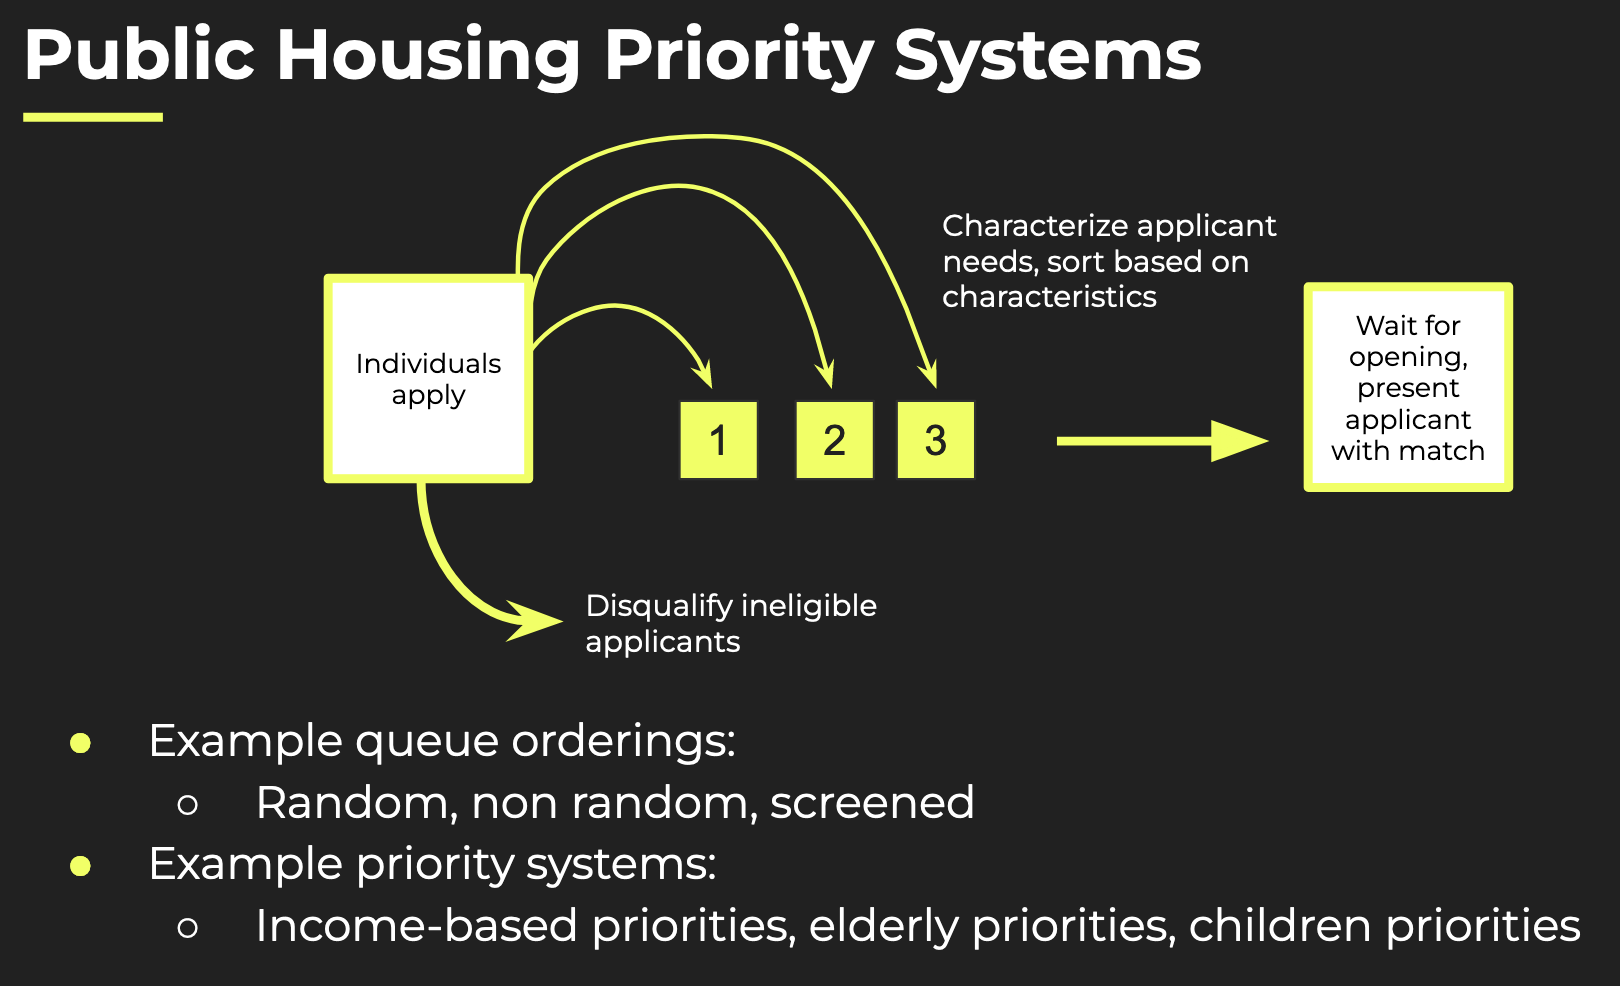
\includegraphics[width=0.75\linewidth]{schematic_priority _systems.png}
    \caption{Diagram of public housing allocation systems}
    \label{fig:schematic}
\end{figure}
\newline
Little is typically known about the methods that cities use to allocate public housing, meaning our first task is to model this process. Using publicly available data on who is awarded housing, we can estimate this process for our chosen city. Relying on estimations made by previous works, we can also integrate assumptions about the rate at which housing becomes available into our predictions to gain a comprehensive approximation of overall public housing availability and allocation. We can apply this model to our city of choice to estimate the flow of applicants in, through, and out of public housing under the city's current system. \\
\newline
With an established model for the present conditions of a city, we can proceed to evaluate alternative allocation systems for fairness. We will apply these alternative systems to our model in order to comment on how the characteristics of tenants shift with the goal of informing future decision making in this sphere. This makes use of a conceptual novelty, in that we expect that ours will be one of the few empirical examinations of fairness implications of choice in housing allocation schemes, as well as a technical novelty in that we will have to develop novel means of approximating allocation mechanisms.
\section{Other related works}
The allocation of scarce resources is a classic problem that pervades social service delivery. At the highest level, prior research has examined the necessity of trade-offs for fairness in social contexts \cite{mashiat2022trade}, arguing that often times many reasonable definitions of equity cannot hold simultaneously. This paper in particular creates a metric of fairness to analyze average realized utility of a resulting outcome, but does not give way to implement allocation systems, which we wish to examine. \\
\newline
There are a variety of studies regarding affordable housing and approximating allocation algorithms. The major limitation of all these studies is that the algorithms are not public. However, Figure 2 describes the general stages of any scheme.\\
\newline
Some papers have abstracted the problem of housing allocation into that of designing waitlists and lotteries \cite{arnosti2020design}. They claim that two approaches of housing allocation create near-optimal matches: independent lotteries and waitlists. They examine in great detail these two modes of allocation, but does not examine the inherent factor of consumer choice in the housing allocation process. Another paper addresses this shortfall by implementing a modified version of the latter of these systems on housing data from Pittsburgh \cite{harvardpublichousing}. Specifically addressing the issue of allocation inefficiency, they argue that implementing an independent waitlist per building reduces the amount of vacant buildings emptied during turnover. However, this algorithm does not account for the nuances of household differences (size, number of children/elderly, veteran status...), which is what we intend to explore. \\
\newline
In our project, we aim to analyze the demographic effects of tenant populations by changing the order of allocations, as in \cite{nyuaffordablehousing}. This paper tackles the issue that housing allocation methods are often unknown and opaque. Thus, they created an algorithm to include priority systems (moving populations with certain characteristics to the front of a queue). Specifically, they analyzed the changes in tenant composition by prioritizing high income households, low income households, the elderly population, and families with children under 18. While the model does shed light on the magnitude of change in these particular orderings, it limits the eligible applicants to those whose household income is above 80\% of the area median income, which severely skews the results. There are also many other key variables such as families with victims of domestic violence, military status, and veteran status that were not explored.\\


\newpage
\section{The Model/Framework}
\noindent
Our city of choice to model policy changes is Baltimore beause of data vailability. With a population of close to 600,000 and a public housing system containing approximately 20,000 properties, Baltimore's robust and widely used public housing system is a suitable choice for analyzing the impacts of differing priority systems on allocation outcomes. \\
\newline
Demand for public housing in Baltimore is also exceedingly high. The public housing system lottery opened for the first time since 2019 in August of 2023, with nearly 30,000 applicants applying during the two week window~\cite{emily_hofstaedter_28000_nodate}. Priority systems are therefore necessary to best allocate the limited available housing to those most in need. \\
\newline

\subsection{Model Data and Privacy Considerations}
\subsubsection{Overview}Our model will employ the 2021 American Community Survey (ACS) microdata~\cite{us_census_bureau_mdat_nodate}. The ACS is an annual survey conducted with the aim of being a nationally representative sample of demographic, economic, and housing information. We will employ demographic variables contained in the ACS data to estimate the number of households eligible for public housing. To gain the most representative demographic variables, we specifically use the 5-year estimates, which average data over a five year period. \\
\newline
Due to the sensitive information collected by the ACS, such as location, income, number of people in households, and so on, privacy considerations exist. Using this data, it could be possible to 'reverse engineer' the survey to gain knowledge about sensitive attributes. For instance, an adversary knowing a family's approximate location and income could use the survey to identify the household's response and gain knowledge about the disability status of the household members. \\
\newline
The ACS has taken steps to mitigate the exposure of sensitive attributes, such as perturbing the attributes uniquely of high income individuals. While the ACS previously hoped to attain differential privacy by 2025, this goal has currently been put on hold~\cite{donna_daily_disclosure_nodate} as a result of internal research finding that a formally private solution currently does not yet exist. Instead, alternative solutions like data perturbations and the inclusion of synthetic data in published ACS reports have been employed. \\
\newline
Because of the existing measures taken by the ACS to preserve privacy, we do not feel that additional measures need to be taken, especially given that our model is reporting only on aggregate demographic changes as a result of different priority systems. However, in real world systems where technology is used in housing allocation, information security should be paramount. City officials should take care to ensure that individual applicant data is stored on secure servers and not susceptible to data breaches to the best of their ability. 
\subsubsection{Data Processing}
After downloading Baltimore City's data from the ACS website, we processed the raw file in R to yield a usable input into our model. We began by selecting only the relevant attributes specified in \autoref{3.2}. From there, we combined individuals into households by serial number and re-coded the data, disqualifying households whose total income exceeded $150\%$ of the poverty line (see Table 2). See the \href{https://github.com/atulpokh/cpsc464final/tree/main}{Github} repository for full code. \\
\newline
We proceed to describe our model, which allocates $M$ housing units to $N$ applicants. 
\subsection{Housing Development Attributes}
Let $M$ be the number of different types of housing units. By the Housing Authority of Baltimore City, public housing authorities manage a little over $M = $ 20,000 units. Each housing unit $m$ is associated with a capacity (number of people who can live in the housing unit). Furthermore, we introduce another parameter $v$ that which represents the general vacancy rate (i.e. how many families leave their affordable housing units per period). \\
\newline
Given this list of $M$ housing units, we also want to determine the number of each unique housing type (in terms of size). Namely, we categorize this list of housing units by their capacity $c$. Let us denote the vector of different types of housing by $\mathcal{M}_u$, where each entry of $\mathcal{M}_u$ represents the number of units for each type of house (number of 1 bedrooms, 2 bedrooms, etc.). \\
\newline
From the most recent annual report, we get the following number of units for each capacity:
\begin{itemize}
    \item 1 Bedroom: $9820$
    \item 2 Bedroom: $4349$
    \item 3 Bedroom: $3107$
    \item 4 Bedroom: $1788$
    \item 5 Bedroom: $880$
    \item 6 Bedroom or More: $569$ 
\end{itemize}
For a total of $20513$ units.

\subsection{Applicant Attributes}
\label{3.2}
Let $N$ be the number of applicants to the housing system. Each applicant $1 \leq i \leq N$ has two vectors associated with it: 
\begin{itemize}
    \item A characteristic vector of length $k = 8$, which represents the $k$ different characteristics (family size, income, race, ethnicity, number of children, number of elderly members, veteran status, disability). We take these attributes from the 2021 5 year ACS survey, filtering by respondents from Baltimore City.
    \begin{itemize}
        \item Family size 
        \item Income
        \item Race of head of household - categorized by (1) White Alone, (2) Black or African American alone, (3) American Indian alone, (4) Alaska Native alone, (5) American Indian and Alaska Native tribes specified, (6) Asian alone, (7) Native Hawaiian and Other Pacific Islander alone, (8) Some Other Race alone, (9) Two or More Races
        \item Ethnicity - (1) Hispanic or Latino, (0) Not Hispanic or Latino
        \item Number of children under 18
        \item Number of elderly over 65
        \item Veteran status of any household members - 1 (True) or 0 (False)
        \item Disability status of any household members - 1 or 0
    \end{itemize}
    Furthermore, in this characteristics table, we add an additional two parameters which we will utilize letter to calculate fairness:
    \begin{itemize}
        \item Wait time - number of periods until the applicant is matched with some housing
        \item Choice number - the ranking of the matched housing unit (i.e. top choice is 1, second choice is 2, ...)
    \end{itemize}
    \item A preference vector $\mathcal{P}_i$ of length $|\mathcal{M}_u|$ that ranks each applicants' preference for each type of housing unit. Recall that each type of housing unit has some capacity $c$. Let us denote the family size of applicant $i$ by $s_i$. \\
    \newline
    We model preferences using the following assumptions: assume that the top preference for every applicant is the housing unit with capacity $s_i$. The following preferences differ by the family size of the applicant, but never exceed $s_i \pm 2$. Thus, every preference vector $\mathcal{P}_i$ will have an ordering of $p \leq 4$ preferences, and the remaining $|\mathcal{M}_u| - p$ entries will be 0. We approximate the housing unit preferences for each applicant (organized by family size) via Table 1.
    \begin{table}[]
        \centering
        \begin{tabular}{c|c|c}
             \text{Family Size} &  Choice 1 & Remaining Choices (in any order)\\
             \hline
             1 & 1 bedroom & 2 bedroom \\
             2 & 2 bedroom & 1, 3, 4 bedroom \\
             3 & 3 bedroom & 1, 2, 4 bedroom \\
             4 & 4 bedroom & 2, 3, 5 bedroom \\
             5 & 5 bedroom & 4, 6+ bedroom \\
             6+ & 6+ bedroom & 5 bedroom
        \end{tabular}
        \caption{Housing Preferences by Family Size}
        \label{tab:my_label}
    \end{table}
\end{itemize} 
\subsection{Housing Allocation Priority Systems}
We consider a variety of possible priority systems, drawing examples from major cities like Cambridge and New York. It's important to note that the list of systems we study is non-exhaustive, rather, it is meant to serve as a baseline approach that could be built upon in real world contexts. The priority systems we consider are as follows:
\begin{enumerate}
    \item \textbf{Priority for households with a member who is disabled.} This priority system recognizes the additional challenges that households with disabled members may face. Allocating resources or benefits to such households ensures a more inclusive and equitable approach, acknowledging the unique needs and support requirements for disabled individuals.
    \item \textbf{Priority for households with a member who is a veteran.} Veterans often face distinct challenges upon returning to civilian life, such as reintegration into the workforce and potential physical or mental health issues. Prioritizing veteran households acknowledges their service to the nation and aims to provide support as they transition back into civilian life.
    \item \textbf{Priority for households with children, ordering those with the most children first.} Children represent the future of society, and supporting households with more children can be seen as an investment in the next generation. This priority system aims to address the financial and logistical challenges that larger families may encounter, ensuring the well-being of children and promoting family stability.
    \item \textbf{Priority for households with elderly members, ordering those with the most first.} Aging populations often require additional care and support. Prioritizing households with more elderly members recognizes the increased potential for health-related needs and aims to enhance the quality of life for older individuals. This approach aligns with a societal commitment to respect and care for the elderly.
    \item \textbf{Priority for households with the lowest income, ordering those households first.} Socioeconomic disparities can significantly impact individuals and families. Prioritizing households with the lowest income addresses the immediate needs of those facing financial hardship. This system aims to reduce inequality and provide essential resources to those who may be most vulnerable in society.

\end{enumerate}
\subsection{Housing Allocation Algorithm}
Consider the following $N$ by $M$ matrix. 
\[H =
\begin{bmatrix}
    \mathcal{P}_1 \\
    \mathcal{P}_2 \\
    \vdots \\
    \mathcal{P}_k
\end{bmatrix}
=
\begin{bmatrix}
    p_{1,1} & p_{1,2} & \cdots & p_{1,M} \\
    p_{2,1} & \ddots & \quad & p_{2,M} \\
    \vdots & \quad & \ddots & \vdots \\
    p_{N,1} & p_{N,2} & \cdots & p_{N,M} 
\end{bmatrix}\]
where $p_{i,j}$ represents the preference ranking for applicant $i$ on housing development $j$. \\
\newline
We introduce two other parameters:
\begin{itemize}
    \item Applicant departure rate $\delta$: at the beginning of each period, we remove $\delta \cdot \texttt{len}(H)$ applicants from the matrix at random. Assume that $\delta$ is constant every period.
    \item Applicant arrival rate $\alpha$: next, we create $X_\alpha \cdot \texttt{len}(H)$ new applicants to add to matrix $H$, where $X_\alpha \sim Poisson(\alpha)$
\end{itemize}
\subsubsection{Data Set-Up}
\begin{enumerate}
    \item We are given $N$ applicants
    \item Generate a $N \times M$ matrix populated with their preference vectors
    \item Eliminate ineligible applicants based on median income. Applicants with household income $150\%$ of the poverty line or below are eligible:
    \begin{table}[htp]
        \centering
        \begin{tabular}{c|c|c}
             \text{Family Size} &  Poverty Guideline & 150\%\\
             \hline
             1 & \$14580 & \$21870 \\
             2 & \$19720 & \$29580 \\
             3 & \$24860 & \$37290 \\
             4 & \$30000 & \$45000 \\
             5 & \$35140 & \$52710 \\
             6 & \$40280 & \$60420 \\
             7 & \$45420 & \$68130 \\
             8 & \$50560 & \$75840 \\
        \end{tabular}
        \caption{2023 Poverty Guidelines in Maryland (Note: after 8 persons, add \$5140 for each additional person) }
        \label{tab:my_label}
    \end{table}
    \item Randomly order the rows
\end{enumerate}

\subsubsection{Initial Data Filtering}
Suppose we are allocating housing by some particularly priority system. For our example, we will use disability.\\
\begin{enumerate}
    \item Create dictionary of housing units available according to \autoref{3.1}.
    \item Remove ineligible applicants (those with median income above $150\%$ of the poverty line)
    \item Move all applicants with characteristic \[\texttt{disability[i] = True}\]
    to the top of the matrix.
\end{enumerate}
\subsubsection{Core Algorithm}
\newline
For each period:
\begin{enumerate}
    \item Apply housing vacancy rate $v$, in other words randomly add
    \[X_v \cdot |M|\]
    different types of housing units.
    where $X_v \sim Poisson(v)$.
    \item Apply applicant departure rate $\delta$. Randomly select $\delta \cdot \texttt{len}(H)$ rows to remove
    \item Apply applicant arrival rate $\alpha$: create $\alpha \cdot \texttt{len}(H)$ new rows and fill with preferences following the same rules described in section 2.
    \item Examine the first row of the matrix
    \item Let us examine the set of plausible housing matches:
    \[J = \{j \mid p_{i,j} > 0\}\]
    \item Choose the column index $j^*$ that that has $p_{i,j^*} = 1$ in $\mathcal{P}_i$. (i.e. choose their top choice of housing)
    \item Examine whether top choice is available (whether the particular housing unit of size $s_i$ is available):
        \begin{itemize}
        \item If available, match applicant $i$ with housing unit of capacity $s_i$. Subtract one from the available units of that size, and mark the choice number of applicant $i$ has 1. Then, remove applicant $i$ from the matrix (remove row $\mathcal{P}_i$)
        \item If not available, proceed to the next ranked housing unit and check for availability. Follow the same rules from the previous step.
        \item If not available and ALL ranked housing units have been checked, move the applicant $i$ to the top of the waitlist and proceed. 
    \end{itemize}
    \item For all applicants $i$ still in matrix $H$, increase their wait time by 1. 
    \item Proceed to the next period. 
    \item Repeat all steps until matrix $H$ is empty or we have run $10^6$ iterations.
\end{enumerate}
Broadly, this process can be visually represented by the image below:
\begin{center}
    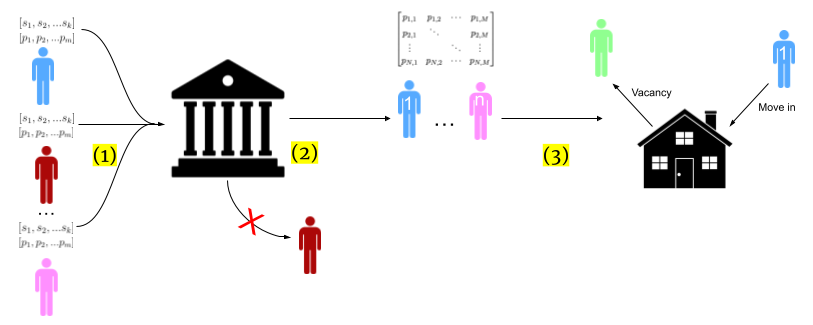
\includegraphics[scale=0.44]{doc/Setup Image.png}
\end{center}
With steps:
\begin{enumerate}
    \item $N$ applicants with characteristic vectors of size $k$ and some preferences (indicated in section 3.2) apply for housing through the government. 
    \item Ineligible applicants are disqualified, while eligible applicants are ordered. Order waitlist based on some priority system.
    \item Applicants are matched to housing as it becomes available. The corresponding row is removed from the matrix and the next applicant becomes first in line.
\end{enumerate}
\begin{algorithm}
\caption{Main Algorithm}
\SetKwInOut{Input}{Input}
\SetKwInOut{Output}{Output}
\Input{Dataframe $df$, Housing units $housing\_units$, Priorities $priorities$}
\Output{New Dataframe $df$ with rankings} 
\ForEach{$priority$ \textbf{in} $priorities$}{
    $df \leftarrow$ original dataframe\;
    \newline
    \eIf{$priority = income$}{
        $waitlist \leftarrow$ sort from low to high income
    }{
        $waitlist \leftarrow$ sort from high to low (number of children, elderly)
    }
    $period \leftarrow 1e6$\;
    \newline
    \For{$\_$ \textbf{in} \text{{range}}(period)}{
        \If{$\text{{waitlist.shape}}[0] = 0$ (waitlist is empty)}{
            \text{{break}}\;
        }
        $housing\_units \leftarrow \text{{housing\_vacancy}}(housing\_units)$\;
        \newline
        \ForEach{$\_, \text{{applicant}}$ \textbf{in} $waitlist.\text{{iterrows}}()$}{
            \newline
            \ForEach{$\text{{rank}}$ \textbf{in} $applicant[preferences]$}{
                \If{$housing\_units[\text{{rank}}] > 0$}{
                    Match applicant to that rank\;
                    \newline
                    Save match to $df[ranking]$\;
                    \newline
                    Update $housing\_units[\text{{rank}}] - 1$\;
                    \newline
                    Remove $applicant$ from $waitlist$
                }
            }
        }
        for $ranking = 0$ applicants, increase $waittime + 1$;
    }
    \newline
    Save statistics and dataframe \;
}
\end{algorithm}
\newpage
\section{Empirical results}
Running our algorithm in Python on the cleaned Baltimore data, we get resulting wait times and probability of top choice for each household. We aggregate these data by racial group and visualize the these metrics for each priority system. \\
\newline
For each trial of the algorithm, we get a set of measures of fairness across groups. Below is an example of fairness measures for one such trial. In these figures, blue bars represent the probability of top choice and red lines represent the average wait time to be housed in periods.
        \begin{table}[h]
            \centering
                \caption{Table of Percentage of Top Choice vs. Average Wait Time for Each Race Group \\
                (Order by priority system: children, disability, elderly, low to high income, veteran status)}
                \vspace{1.1em}
                \begin{tabular}{cc}
                    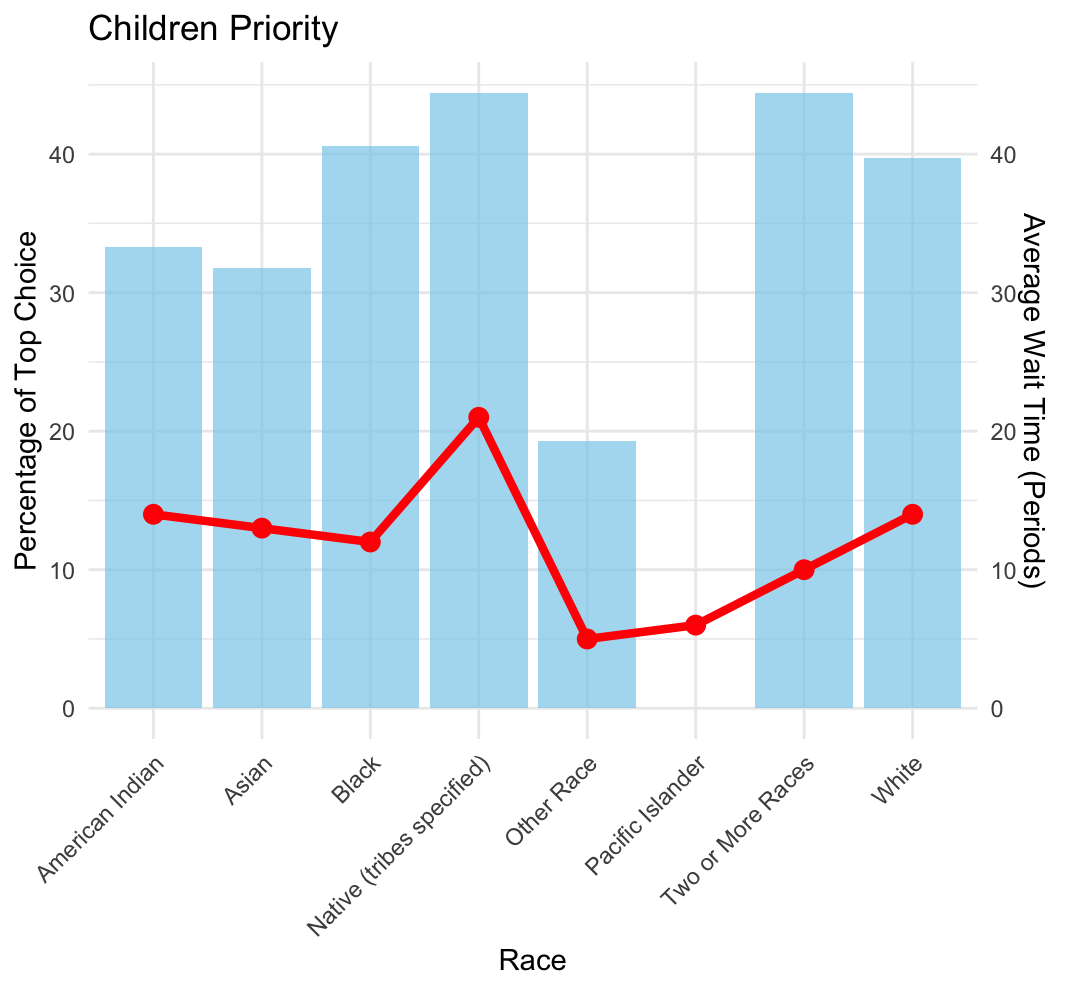
\includegraphics[width=0.33\linewidth]{Children.png}
                    & 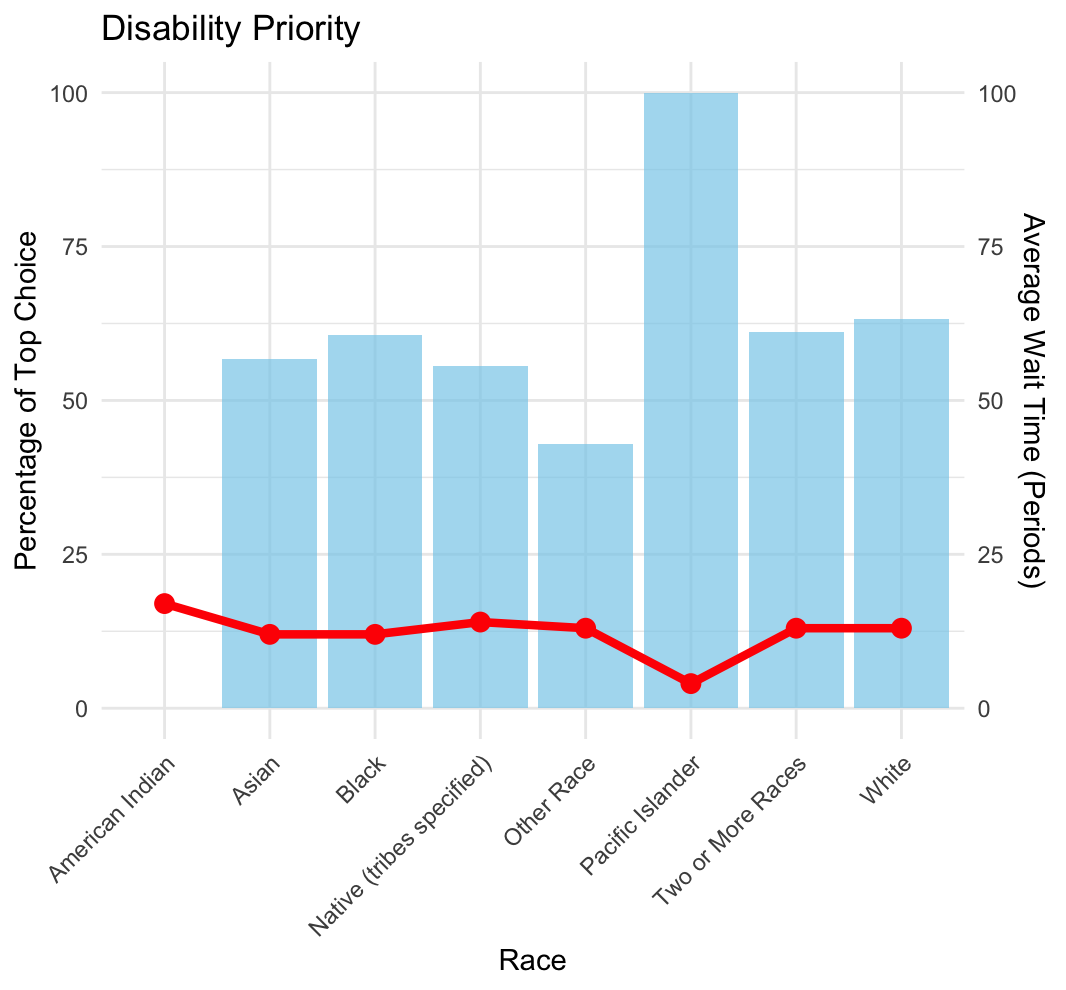
\includegraphics[width=0.33\linewidth]{Disability.png} \\[-4pt]
                    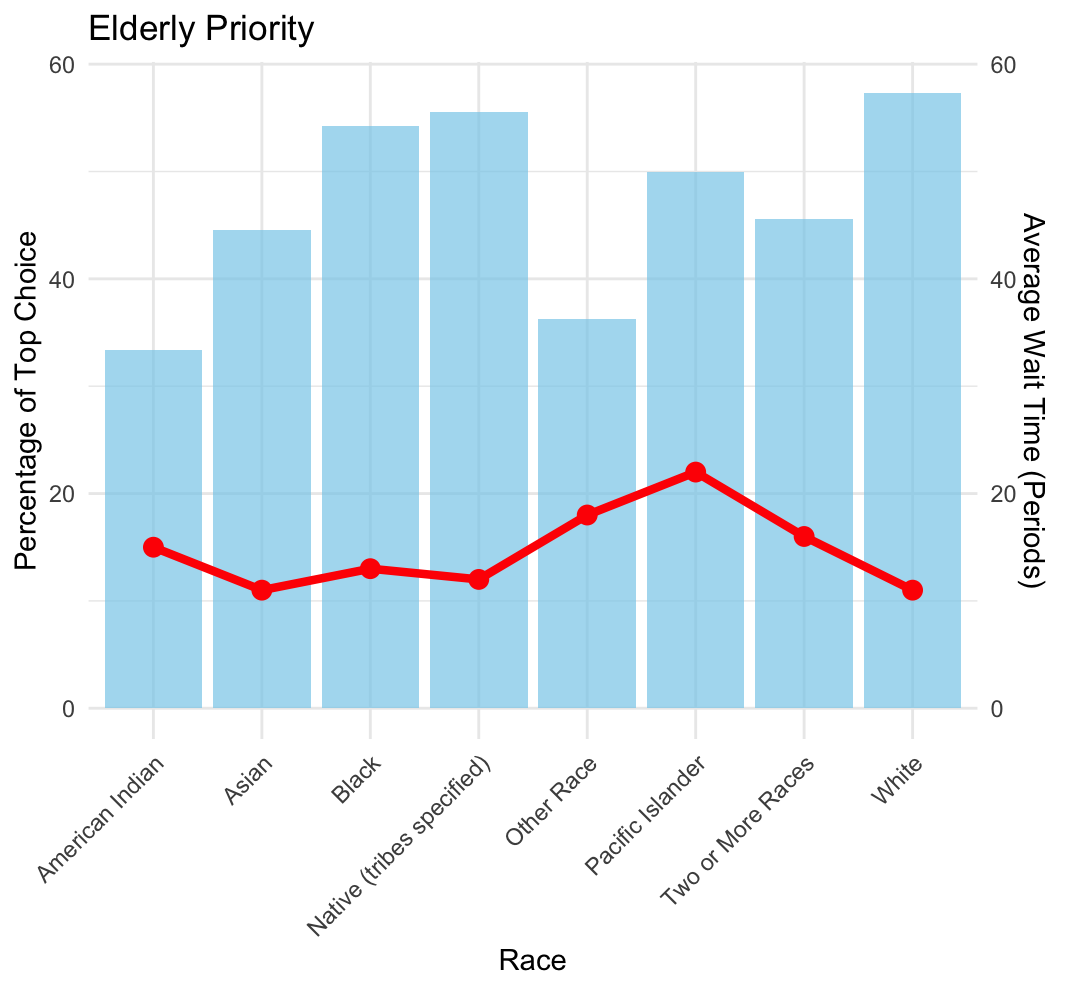
\includegraphics[width=0.33\linewidth]{Elderly.png} & 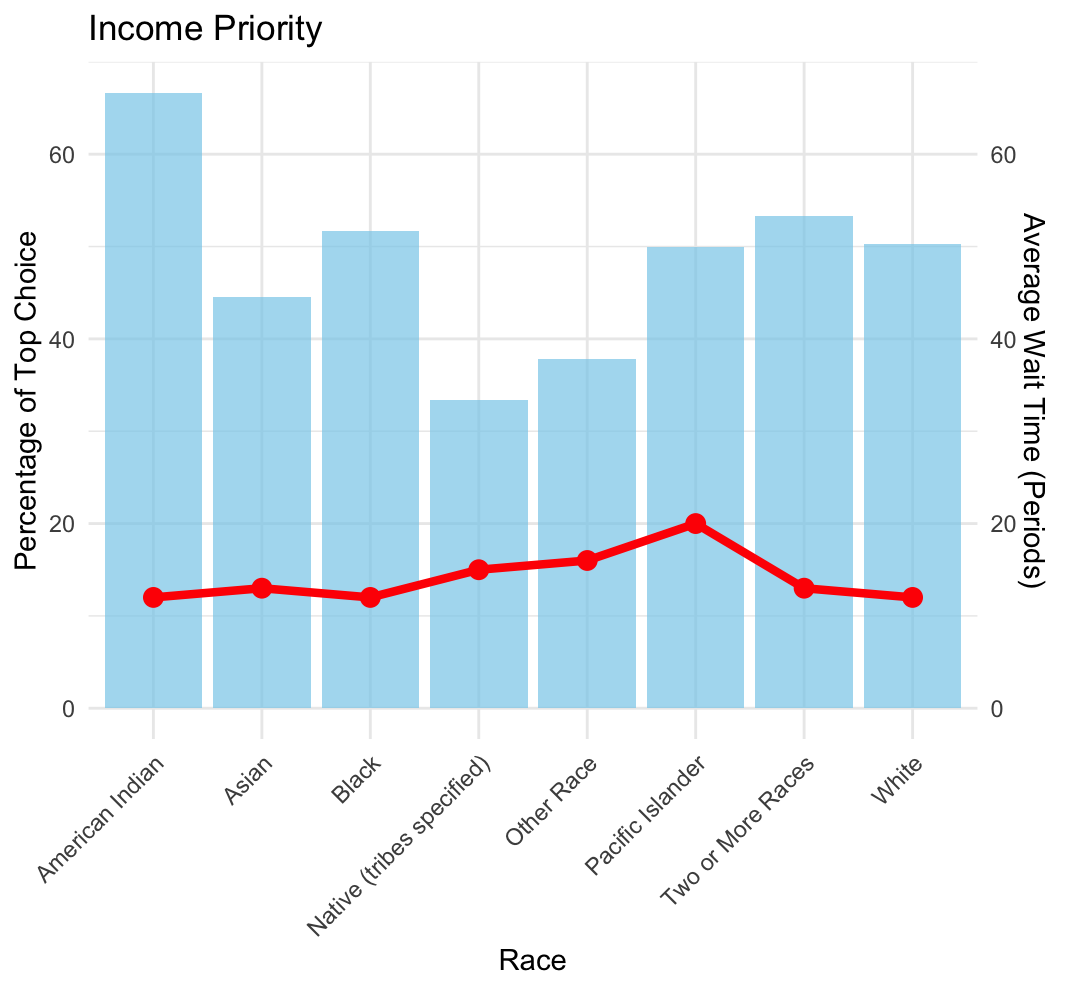
\includegraphics[width=0.33\linewidth]{Income.png} 
                \end{tabular}%
        \end{table}
\[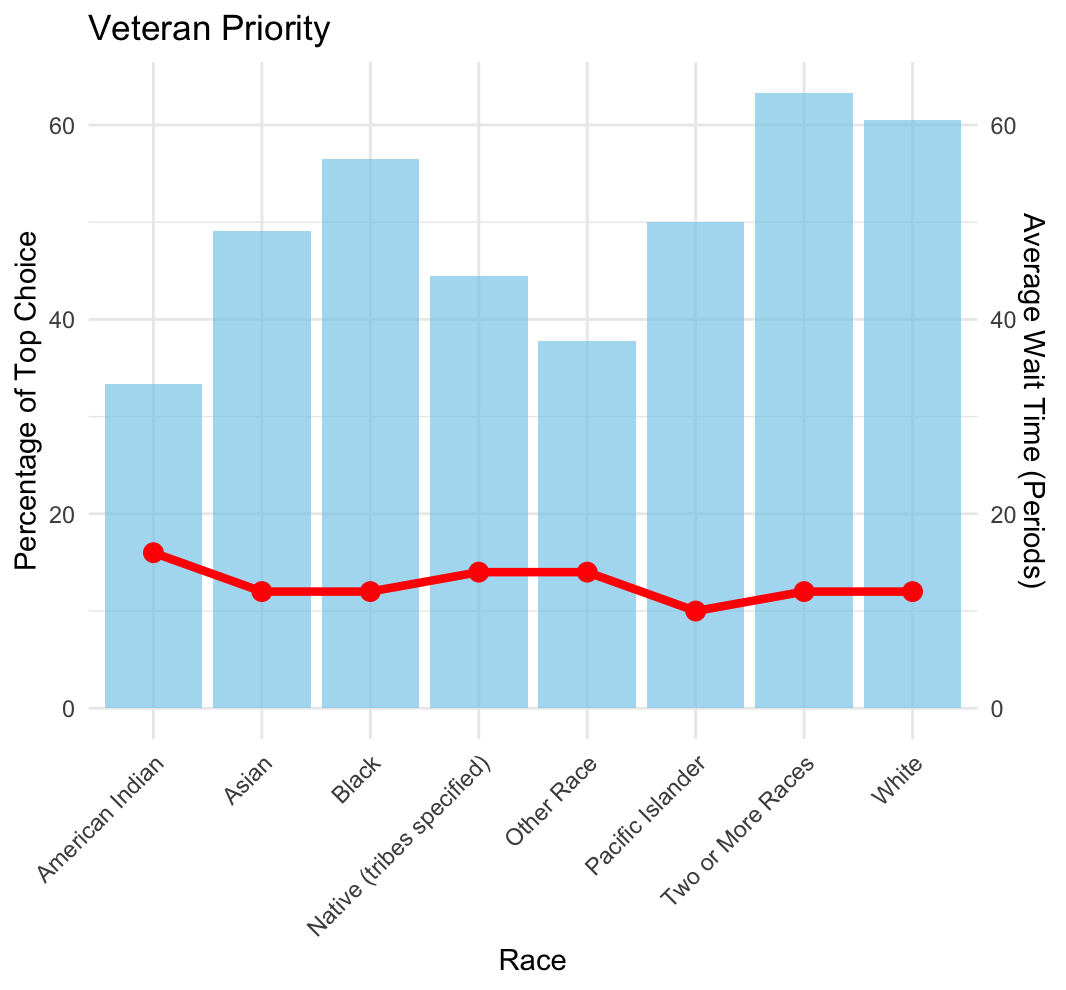
\includegraphics[width=0.33\linewidth]{Veteran.png}\]
Running the simulation 


 \begin{table}[h]
            \centering
                \caption{Distribution of top choice percentage by racial group and priority (10 experiments)\\
                (Order by priority system: children, disability, elderly, low to high income, veteran status)}
                \vspace{1.1em}
                \begin{tabular}{cc}
                    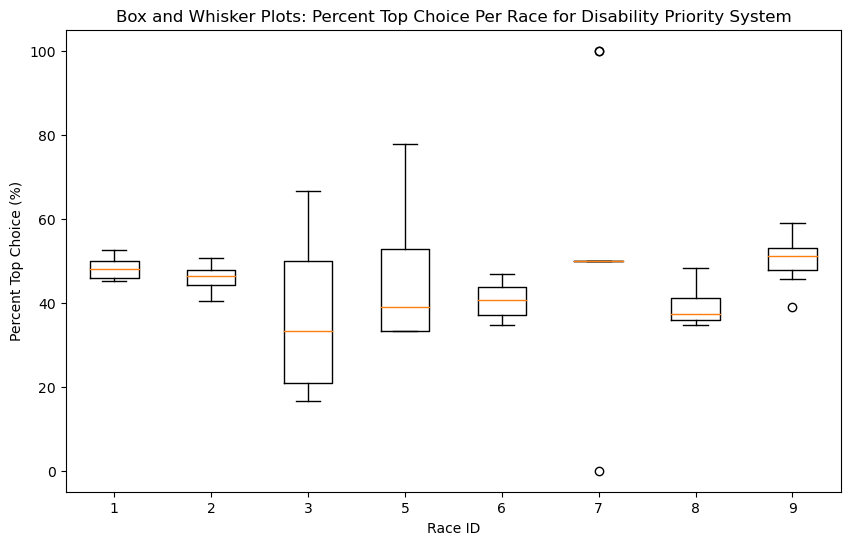
\includegraphics[width=0.5\linewidth]{doc/FinalReport/tcp1.png}
                    & 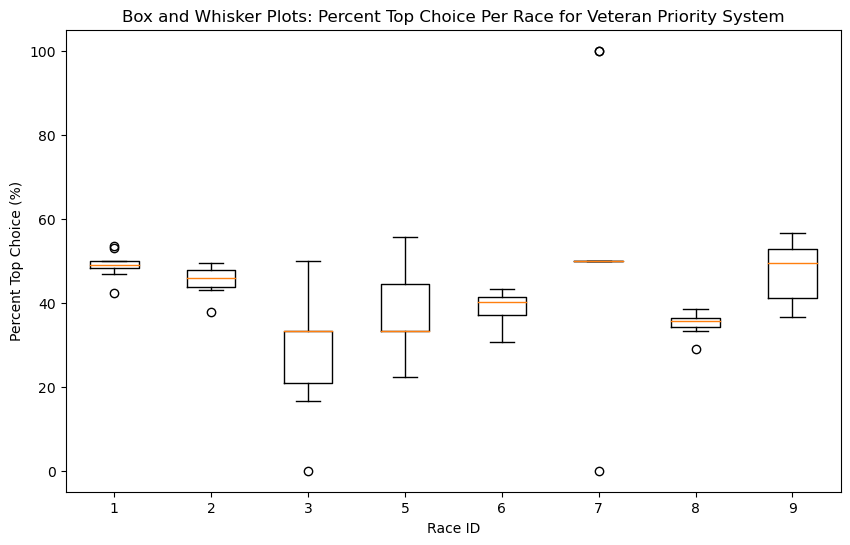
\includegraphics[width=0.5\linewidth]{doc/FinalReport/tcp2.png} \\[-4pt]
                    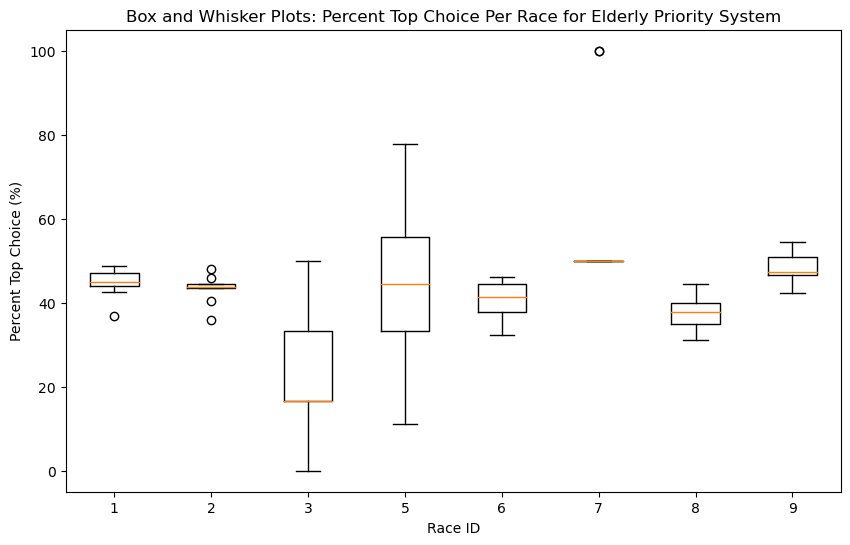
\includegraphics[width=0.5\linewidth]{doc/FinalReport/tcp3.png} & 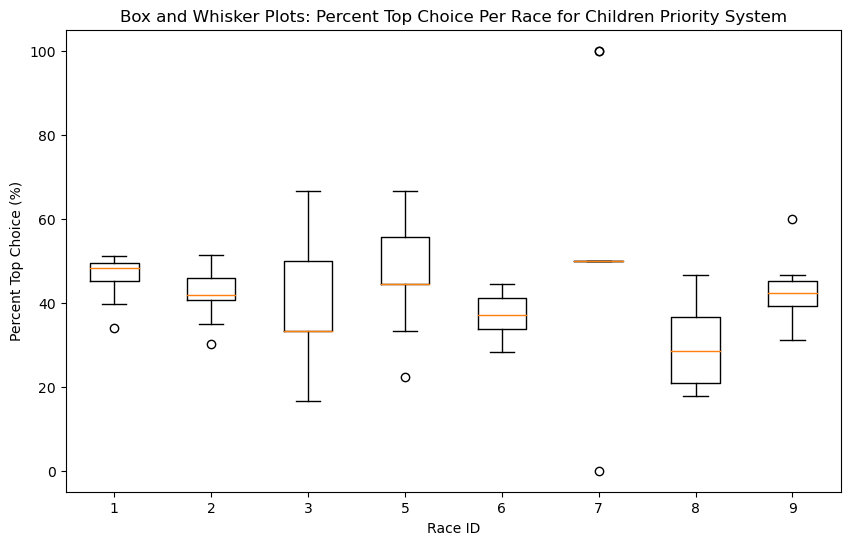
\includegraphics[width=0.5\linewidth]{doc/FinalReport/tcp4.png} 
                \end{tabular}%
        \end{table}
\[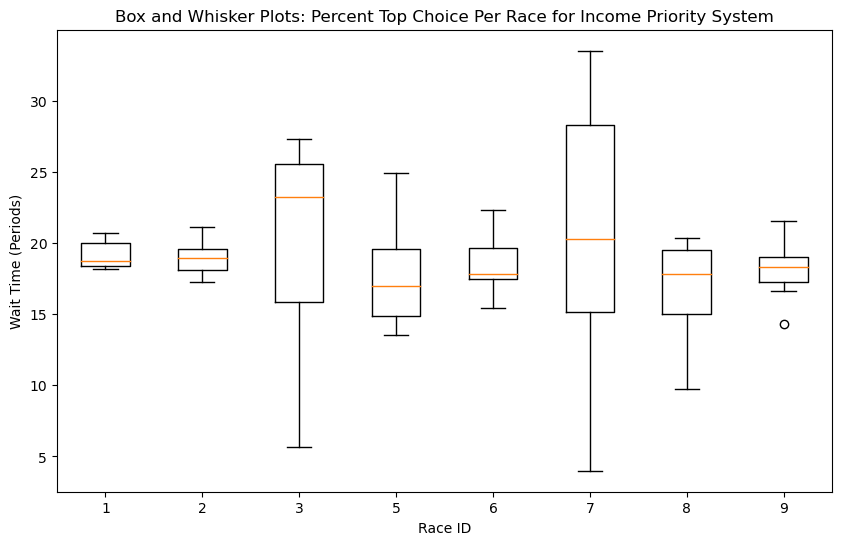
\includegraphics[width=0.5\linewidth]{tcp5.png}\]

\section{(Desired) Theoretical results}

\subsection{Measurement of Fairness}

Since algorithm design is ultimately a human-driven process, we intend to introduce measures
of fairness to track different applications of our priority system. Notedly, data collection was conducted externally, so its particular impact on the algorithm’s fairness assessment cannot be discerned. Furthermore, though there is no classifier that can handle all notions of fairness, previous study has been done on the fairness in allocation systems.

For instance, Jo, Tang, Dullerud, Sina Aghaei, Rice, and Vayanos (2022) \cite{formulaeval3} propose a framework
for fairness evaluation in contextual resource allocation systems that is inspired by fairness
metrics in machine learning. They find that there is often incompatibility between allocation
fairness and outcome fairness. In other words, the distribution mechanism itself may be fair,
even if end results are not equitably distributed. They also conclude that “policies that prioritize based on a vulnerability score will usually result in unequal outcomes across groups, even if the score is perfectly calibrated.” This is relevant in our consideration of priority characteristics.

Next, Rodolfa, Lamba, and Ghani (2021) \cite{formulaeval2} explain the importance of algorithms being sensitive to
the possible worsening of pre-existing inequalities upon their implementation; this introduces the idea of temporal fairness analysis. Lastly, Bunce, Richardson, et al. (2021) \cite{formulaeval} review CBDG,
HUD's best-known formula for allocating 3.3 billion USD of federal funds to 1,239 jurisdictions. They find that over the past 50 years, “equity under the current CDBG formula has considerably worsened, [...] the formula still provides more funding per capita to higher-need communities than to lower-need communities.” To determine if this is the case with our algorithm, we introduce two measures of fairness.

\subsubsection{Average Wait Time}
Let $H_1, H_2, \dots, H_\ell$ be subsets of our data, grouped by some characteristic $S_k$. Furthermore, for every applicant $X \in H_k$, let $T_i$ represent the wait time of the applicant $i$ and $t_k$ be the average wait time of applicants in the $k$-th subset. Namely,
\[t_k = \frac{1}{|H_k|}\sum_{i=1}^{|H_k|}T_i\]
Then, we calculate fairness by calculating average wait time for each subset $H_k$, which is organized by characteristic $S_k$. We want $S_k$ and the characteristic used for the priority system to be \text{different}. Then, we measure fairness by the equality group fairness metric:
\[\text{minimize}(t_i - t_j) \quad \text{ for } i \neq j\]
\subsubsection{Probability of Top Housing Choice}
We introduce another metric of fairness that determines the probability that a certain group gets their top housing choice. \\
\newline
Similarly, let $H_1, H_2, \dots, H_\ell$ be subsets of our data, grouped by some characteristic $S_k$. Recall that each applicant has a characteristic $Y_k$ which tracks their choice number (i.e. whether they got their top choice, second choice, etc.) \\
\newline
Then, we calculate fairness by calculating the probability that an applicant in $H_k$ is matched with their top housing choice. Namely, we measure fairness by aiming to achieve:
\[\frac{P(Y = 1 | H_i)}{P(Y = 1 | H_j)} = 1 \quad \text{ for } i \neq j\]

Algorithms naturally encode human biases, so having an empirical set of fairness definitions provides a testing regime for how our proposed ranking system compares to others. These definitions are a more reliable metric than simply assuming diversity implies fairness. 

\subsection{Model Evaluation}
Taking the results and discussed above, we consider how each allocation preforms overall in terms of how many people get their top choice and the average wait time. In this case we would gravitate towards priority systems which award a higher percentage of people their number one choice, as well as systems with the lowest average wait time. \\
\newline
Using the fairness metrics discussed above, we consider the fairness of each priority system, using race as our grouping characteristic. Each fairness column is calculated by
$$
\biggr{|}1 - \frac{1}{(n^2 - n)}\sum_i \sum_j \frac{X[i]}{X[j]}\biggr{|} \quad \text{ for } i \neq j\
$$
where $X$ is a vector of either average wait time or average percent of top choice, and each index of $X$ represents a different racial group. Essentially, this is an average of the ratio of group to group fairness measures for each possible group combination. Lower measures of this metric are better, as they indicate a higher degree of fairness across racial groups for percentage of top choice and average wait time. Note that values of zero are omitted when preforming this calculation.\\
\newline
The results of this analysis are below:
    \begin{table}[H]
        \centering
        \begin{tabular}{c|c|c|c|c}
             Priority &  Average \% Top Choice & Average Waittime & Top Choice Fairness & Average Waittime Fairness \\
             \hline
             Disability & \textcolor{blue}{55.025\%} & 12.25 & 0.08651679 & \textcolor{blue}{0.06583475}\\
             Income & 48.45375\% & 14.125 & 0.08379766 &  0.09561799\\
             Children & 31.6875\% & \textcolor{blue}{11.875} & \textcolor{blue}{0.06552772} &  0.08832704 \\
             Eldery & 47.10125\% & 14.75 & 0.08963984 & 0.06991156 \\
             Veteran & 49.3775\% & 12.75 & 0.07978653 & 0.1070871 \\
        \end{tabular}
        \caption{Overall average and fairness measures by racial group. Lowest values are indicated in blue.}
        \label{tab:my_label}
    \end{table}
\newline
These results offer insights into the performance and fairness of each priority system:
\begin{itemize}
    \item Disability Priority: This system achieves an impressive average percentage of top choice ({55.025\%}), coupled with a relatively low average wait time of 12.25. The fairness measures for both top choice and average wait time, indicated in blue ({0.08651679} and {0.06583475} respectively), suggest a commendable level of equity among racial groups.
    \item Income Priority: While the average percentage of top choice is lower (48.45375\%), the associated fairness measures (0.08379766 for top choice and 0.09561799 for average wait time) indicate a reasonable level of equity in allocation across racial groups.
    \item Children Priority: This system exhibits a lower average percentage of top choice (31.6875\%), but the fairness measures, especially the lowest values indicated in blue ({0.06552772} for top choice and 0.08832704 for average wait time), highlight a higher degree of fairness, particularly in terms of average wait time.
    \item Elderly Priority: With a relatively high average percentage of top choice (47.10125\%) and fairness measures of 0.08963984 for top choice and 0.06991156 for average wait time, this system demonstrates a reasonable balance between performance and fairness.
    \item Veteran Priority: While the average percentage of top choice is competitive (49.3775\%), the associated fairness measures (0.07978653 for top choice and 0.1070871 for average wait time) suggest a need for further examination to enhance equity, particularly in terms of average wait time.
\end{itemize}
\newline
In summary, the Disability and Elderly priority systems emerge as strong performers, achieving high average percentages of top choice while maintaining a commendable level of fairness across racial groups. Further investigation and potential adjustments are warranted for the Children and Veteran priority systems to address observed disparities in fairness metrics.

\section{Next Steps, Limitations, and Future Work}
A particularly salient area of future research considers consumer choice after considering the utility (perceived and actual) of their allocated public housing unit. This is useful in further making the ranking system more fair and efficient, so that more families accepts their initial housing draw – that is, through maximizing utility, each applicant(s) should be matched with housing that most suits their preferences so they don’t take up space for multiple units, or have to return to the waitlist after being being matched with an unsatisfactory unit. \\
\newline
In the past, families have been actively encouraged to apply to units in multiple locations to maximize their overall chance of being matched with housing. Though the average number of housing applications an American family submits is unknown, housing portals state, “The more lists you’re on, the higher your chances of being awarded a housing choice voucher” ~\cite{advisors_stuck_2023}. This complexity has contributed to an increasing amount of time between tenants as agencies simultaneously hold different units for the same person, who will, ultimately, only choose the best unit. This extends the waiting time for everyone as that same applicant gets screened and contacted (both being time-intensive processes) for each of the various units they applied for. The Agawam Housing Authority in Massachusetts, for instance, reports that it takes years to find a new tenant, as hundreds of names must be analyzed before a match is found~\cite{todd_wallack_mass_2023} . Scenarios like this result in phenomena like in the nearby town of Gardner, Massachusetts which has a vacancy rate of 21\%, meaning 70 out of 342 units are vacant even as the waitlist contains 11,775 people~\cite{todd_wallack_mass_2023} . On a national scale, the Public Housing Dashboard put out by the HUD reveals that there is a lesser, though still significant vacancy rate of five percent~\cite{hud_public_nodate}. Northwestern states like Oregon, Washington, and Idaho have higher-than-average occupancy rates while Kansas and Maryland have sub-90\% occupancy rates. All things considered, having any vacant unit can be considered a failure of the matching algorithm and have significant societal implications. \\
\newline
While determining if an algorithm maximizes utility initially seems like an especially useful mechanism for evaluating an algorithm’s fairness, it comes with certain drawbacks and limited technical feasibility. The first is that it, like many other fairness measures, relies on highly accurate data. However, inaccuracies can arise through human data entry leading to incorrect documentation of familial characteristics (e.g. number of children) or lack of up-to-date information on the state of or vacancy of housing (e.g. whether or not it is occupied or under renovation, thus unavailable). The curation of the former and maintenance of the latter is resource-intensive from a financial and human capital perspective. \\
\newline
Further bias can arise from the assumption that certain familiar characteristics align with preference for certain housing, i.e. assuming that families with more children prefer larger housing units. If an empirical way to collect these preferences is indeed established, it has to account for context drift or familial circumstances and preference changing over prolonged waiting times \cite{conceptdrift}. \\
\newline
In conclusion, these obstacles serve as a reminder that the design of algorithms is intrinsically linked with human decision-making and subjectivity \cite{humanerror}. Technical improvements and considerations of the societal implications of the algorithms used in housing policies are only part of the process of ensuring fairer housing allocation in places like Baltimore. After all, historic housing policy decisions play a leading part in dictating the effectiveness of current policy efforts. We hope this paper encourages broader and more thoughtful discussion on the usage of computer science in improving the lives of urban dwellers. 


\newpage
\bibliographystyle{plain}
\bibliography{references} 


\end{document}
